\begin{figure}
\section{Namespace-Übersicht}
    \centering
    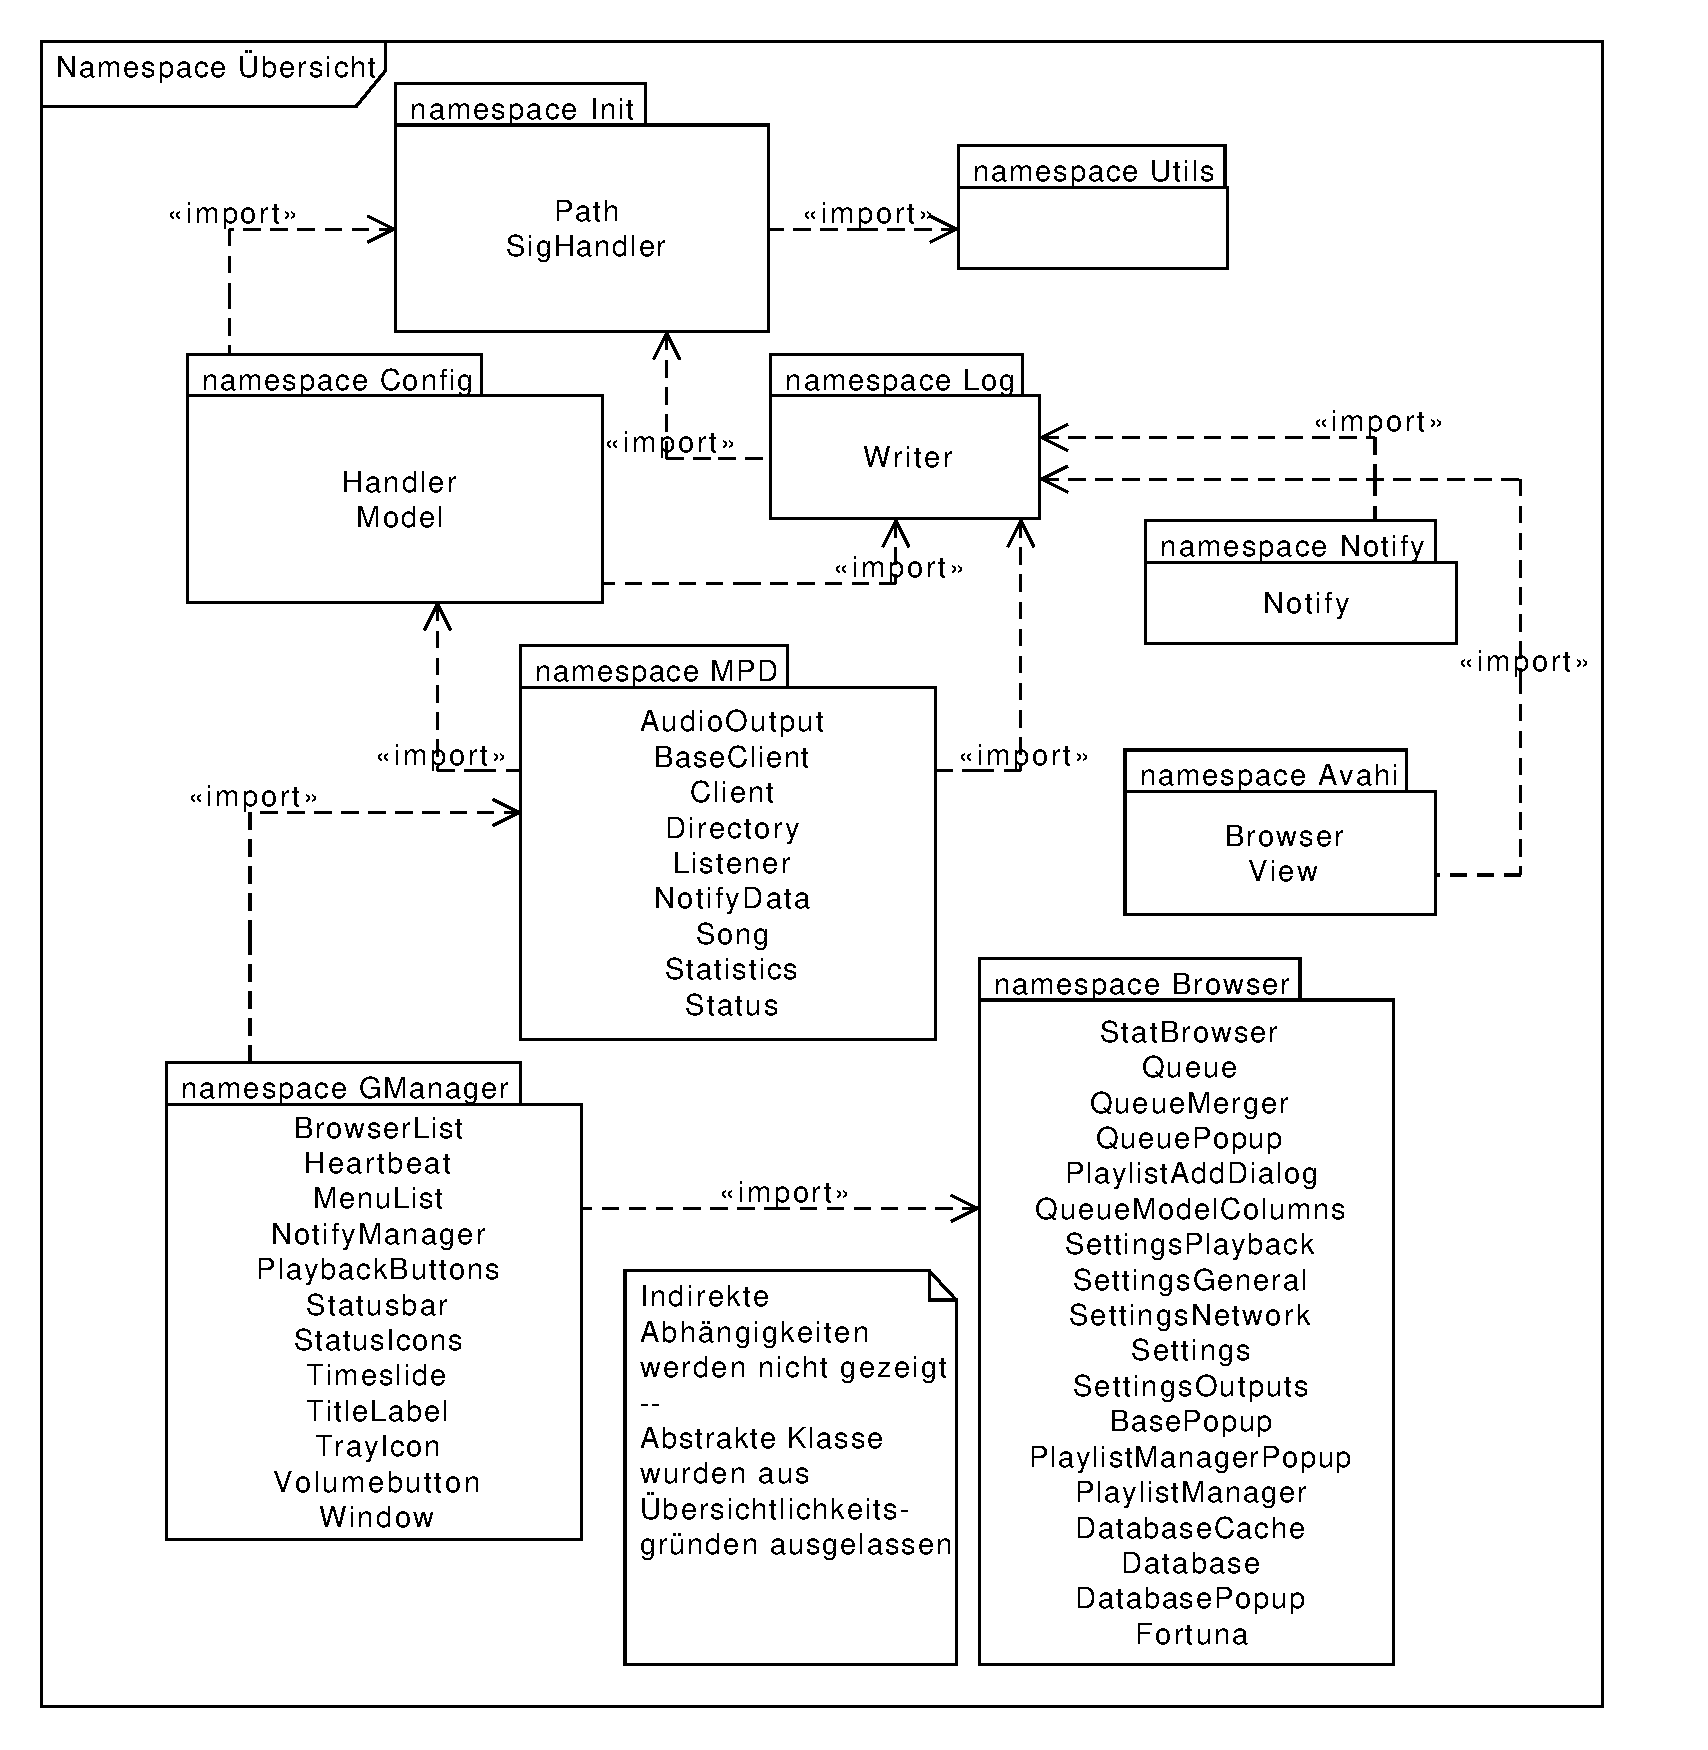
\includegraphics[scale=0.50]{./gfx/class/package}
    \caption{Die Namespaces im Überblick}
    \label{dd_namespaces}
\end{figure}

\begin{figure}
\section{Aufbau der Anwendung}
	\centering
        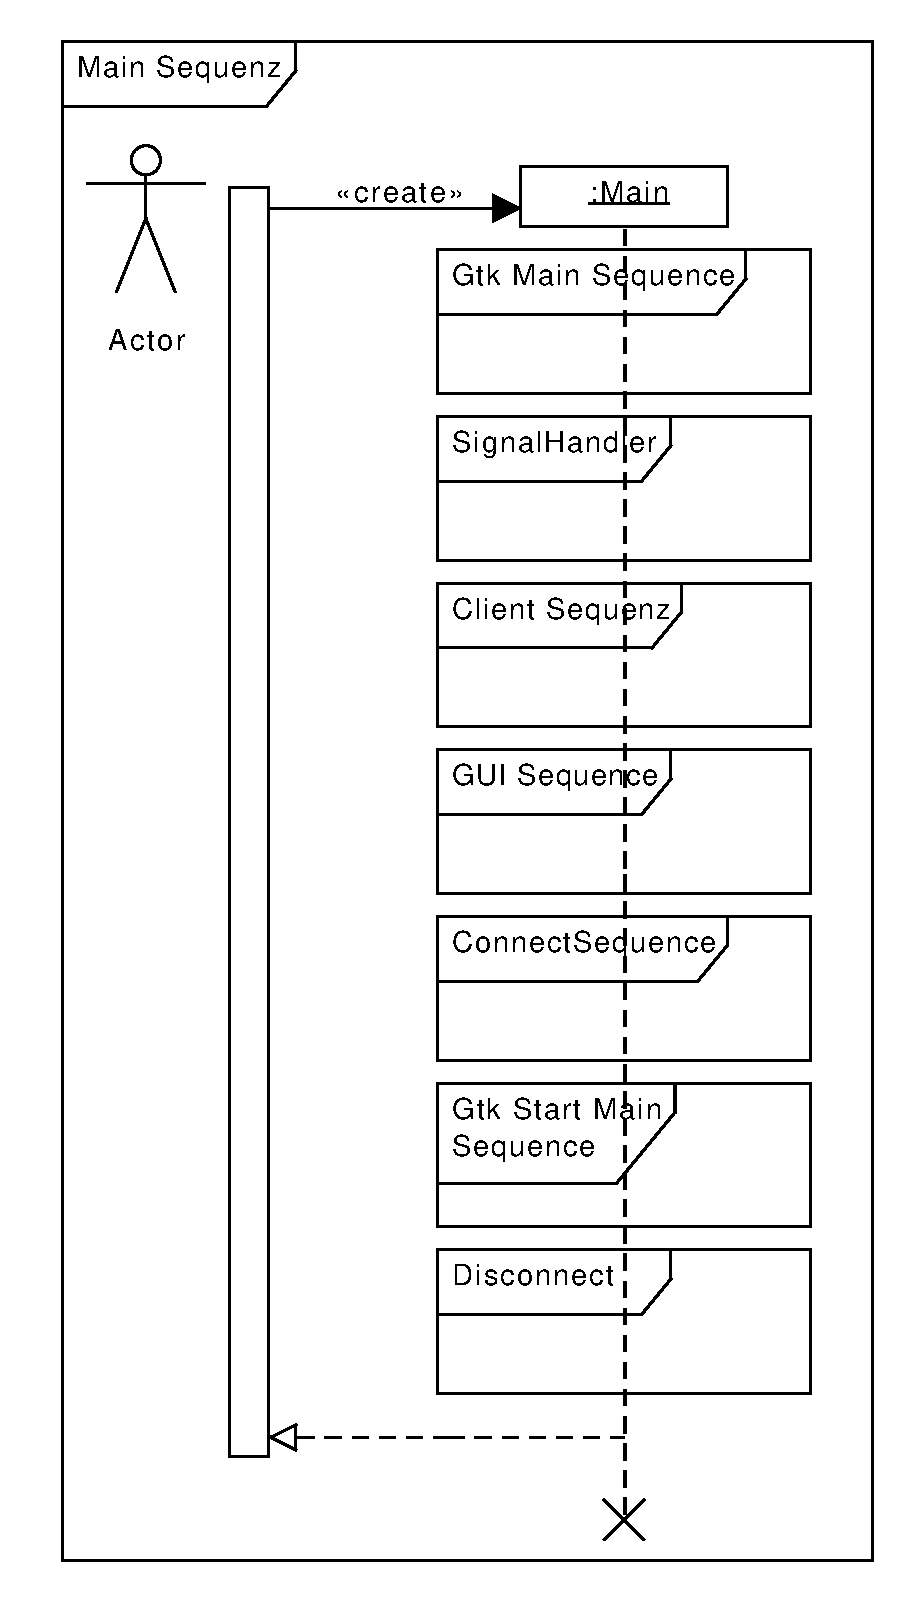
\includegraphics[scale=0.5]{./gfx/seq/main}
	\caption{Die Initialisierungsphase}
	\label{seq_main_init}
\end{figure}





\section{Utils und Writer} 

\subsection{Utils}
Im \emph{Utils Namespace} sollen sollen sich folgende Hilfsfunktionen zur Zeit/Datumsumrechnung befinden:

\begin{itemize}
    \item Umrechnung von Sekunden in einen ,,Dauer-String Bsp'' : ,,4 hours 2 minutes 0 seconds''

        \begin{verbatim}
        Glib::ustring seconds_to_duration(unsigned long);
        \end{verbatim}

    \item Umrechnung Sekunden in einen Timestamp, Bsp: ,,2011-04-02''
        \begin{verbatim}
        Glib::ustring seconds_to_timestamp(const long);
        \end{verbatim}

    \item Umwandlung eines Integer Wertes in einen String
        \begin{verbatim}
        std::string int_to_string(int num);
        \end{verbatim}
\end{itemize}


Diese grundlegenden Funktionen sollen ausgelagert werden damit sie von mehreren Klassen verwendet werden können und um Redundanzen im 
Code zu vermeiden.

\subsection{Logging}
\begin{figure}[htb!]
    \centering
    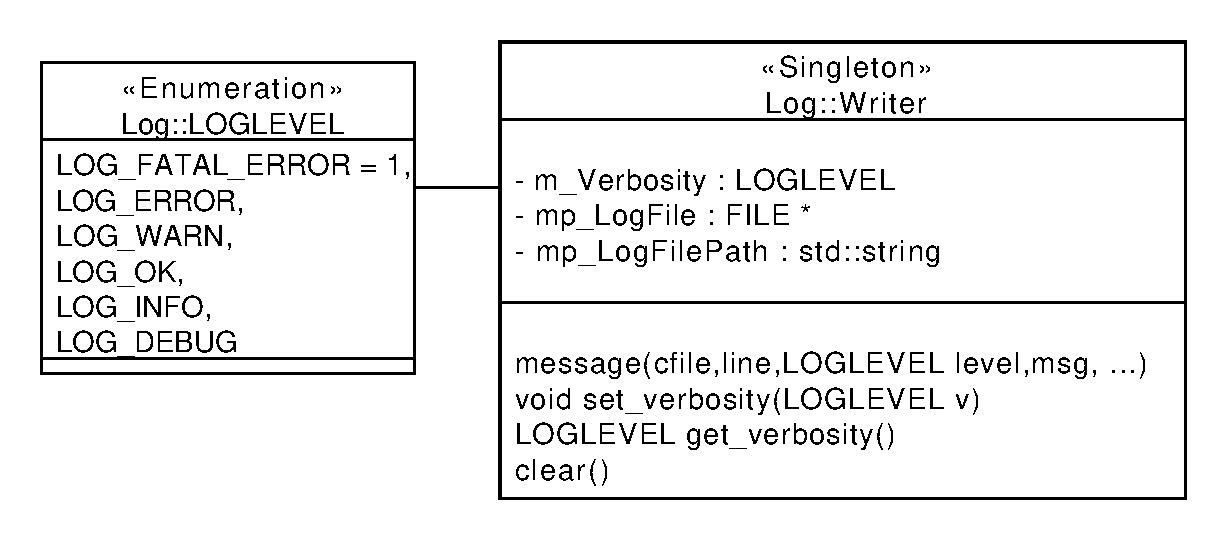
\includegraphics[scale=0.6]{./gfx/class/log}
    \caption{Klassendiagramm zu Log::Writer}
    \label{c_log}
\end{figure}
Im \emph{Log Namespace} befindet sich die Writer Klasse, welche auch als sog. ,,\textit{Utils-Klasse}'' Funktionen für alle anderen
Klassen in Namespace bereitstellt. Bei dieser Klasse wurde das Singleton Pattern gewählt, damit sie leicht von ,,überall'' aus erreichbar ist, ohne dass vorher explizit eine Instanzierung statt finden muss. Die Logdatei wird im Konfigurationsverzeichnis von Freya als log.txt
abgespeichert, im folgenden Dokument gibts dazu mehr Informationen. 
Die Logklasse dient zur Protokollierung von Fehlern und besonderen Ereignissen.  

\begin{figure}[htb!]
    Folgende selbsterklärende Makros werden von der \emph{Log::Writer} Klasse zur Protokollierung bereitgestellt:

  \begin{verbatim}
  _MSG(level, msg, ...) Log::Writer::instance().message(level, ...)

  Fatal(msg, ...)    _MSG(Log::LOG_FATAL_ERROR, msg, ...)
  Error(msg, ...)    _MSG(Log::LOG_ERROR, msg, ...)
  Warning(msg, ...)  _MSG(Log::LOG_WARN, msg, ...)
  Success(msg, ...)  _MSG(Log::LOG_OK, msg, ...)
  Info(msg, ...)     _MSG(Log::LOG_INFO, msg, ...)
  Debug(msg, ...)    _MSG(Log::LOG_DEBUG, msg, ...)
  \end{verbatim}
\end{figure}

Als weitere Funktionalität soll beim instanzieren geprüft werden ob die Größe der Logdate 2MB überschreitet. In diesem Fall soll die Logdatei neu angelegt werden.
Um die ,,Gesprächigkeit'' (Verbosity) der Logklasse zu kontrollieren sollen zudem folgende Makros geboten werden:
\begin{verbatim}
 LogSetVerbosity(LV) Log::Writer::instance().set_verbosity((Log::LOGLEVEL)LV)
 LogGetVerbosity     Log::Writer::instance().get_verbosity()
\end{verbatim}
Die höchste Gesprächigkeit hat dabei \emph{Log::FATAL\_ERROR}, die niedrigste \emph{Log::LOG\_DEBUG}. Wird also beispielsweise LogSetVerbosity(\emph{Log::LOG\_WARN}) aufgerufen, so
werden nur noch fatale Fehler, Fehler und Warnungen ausgegeben. Die Reihenfolge entspricht den Makros weiter oben.
Soll die Ausgabe vollkommen abgeschalten werden so kann eine Zahl kleiner 1 an LogSetVerbosity() übergeben werden.

%----------------------------------------------------------------------------------------------

\section{Config Hauptklassen}

\subsection{Path}
Die \emph{Init::Path} Klasse soll für die Initialisierung und das Management der Freya Config Pfade zuständig sein.
Bei der Initialisierung soll überprüft werden ob das Konfigurationsverzeichnis vorhanden ist, wenn nicht wird ein Neues
angelegt und anschließend wird eine default config.xml geschrieben. Eine Standardkonfiguration ist im Quellcode als 
konstanter globaler String einkompiliert.
\\
\\
Schlägt das Erstellen der Konfigurationsdatei fehl, so soll versucht werden eine entsprechende Fehlermeldung in die Log Datei zu schreiben, 
falls diese zuvor erfolgreich angelegt wurde. Zusätzlich sollen DEBUG Ausgaben auf dem Bildschirm angezeigt werden, wenn das Programm
über ein Terminal gestartet wird.

\paragraph{Instanzierung der Path Klasse kurz erläutert:}
Bei der Instanzierung werden die private Methoden get\_config\_dir() und get\_config\_path() aufgerufen, deren Rückgabewerte werden
als Membervariablen der Init::Path gespeichert. Diese Methoden nutzen die g\_get\_user\_config\_dir() glib Methode
welche den User Pfad nach XDG Standard zurückliefert.\footnote{http://standards.freedesktop.org/basedir-spec/basedir-spec-latest.html}
\\
\\
Je nach Funktion, wird an den Pfad ein ,,/freya'' für das Freya Konfigurationsverzeichnis, ,,config.xml''
für die Konfigurationsdatei oder ,,log.txt'' für die Logdatei dran gehängt.
\\
\\
Bei der Initialisierung wird die dir\_is\_avaiable()
Methode aufgerufen. Diese prüft ob die nötigen Verzeichnisse und Dateien existieren, wenn nicht wird versucht diese
anzulegen. Diese Klasse schreibt DEBUG und ERROR Ausgaben auf die Konsole raus, da zum Zeitpunkt der Initialisierung
nicht gewährleistet werden kann dass eine Logdatei existiert.


\paragraph{Die ,,dir is available()'' Methode kurz erläutert:}
Diese Methode prüft zuerst über die glib Funktione g\_file\_test() ob ein ,,freya'' Verzeichnis existiert,
ist dies nicht der Fall werden die privaten Methoden create\_dir() und create\_config() aufgerufen.
Ist ein ,,freya'' Verzeichnis vorhanden, so wird über die glib g\_file\_test() Funktion geprüft ob die Konfigurationsdatei
config.xml existiert. Existiert diese nicht, so wird die private create\_config Methode() aufgerufen.
Existiert diese, so wird mittels der glib g\_access() Methode geschaut ob diese lesbar und beschreibar ist. 
Bei Misserfolg wird über die glib Funktion g\_warning eine entsprechende Fehlermeldung auf
dem Bildschirm (Konsole) ausgegeben, da die Logklasse zu diesem Zeitpunkt noch nicht aufgebaut worden ist.


\paragraph{Die ,,create config()'' Methode kurz erläutert:}
Die Mothode soll zum Anlegen eines Konfigurationsverzeichnisses verwendet werden.
Im Fehlerfall wird eine entsprechende Warnung über glib Funktion g\_warning() auf dem Bildschirm ausgegeben.

\paragraph{Die ,,create dir()'' Methode erläutert:}
Diese Methode bietet die Funktionalität über die glib Funktion g\_mkdir\_with\_parents(configdir,0755) ein Verzeichnis mit den rechten 755 (drwxr-r-xr-x) anzulegen. Bei Erfolg wird mit g\_message() eine Erfolgsmeldung auf dem Bildschirm (Konsole)
ausgegeben, andernfalls eine warnung mit g\_warning().


%----------------------------------------------------------------------------------------------

\subsection{Konfigurationsdatei}

Die Freya Konfigurationsdatei soll im simplen XML Format realisiert werden, XML wird gewählt um das Parsen zu vereinfachen und um
ein standardisiertes Format nach außen bereitzustellen. 
\\
Die Konfigurations- und Logdatei soll nach XDG Standard \verb+($XDG_CONFIG_HOME)+ unter \verb+$HOME/.config/freya/<config.xml,log.txt>+ gespeichert werden.

\begin{itemize}
    \item \url{http://standards.freedesktop.org/basedir-spec/basedir-spec-latest.html#variables}
\end{itemize}

Die Optionen in der Konfigurationsdatei sind baumartig nach ,,Domainprinzip'' aufgebaut. Die Konfigurationsdatei unter \ref{c_config}
zeigt exemplarisch den gewünschten Aufbau.
\begin{figure}[htb!]
    \lstinputlisting[language=XML]{./src/config.xml}
    \caption{Config.xml Konfigurationsdatei im Überblick}
    \label{c_config}
\end{figure}


\newpage
\subsection{Model}
\begin{figure}[htb!]
    \centering
    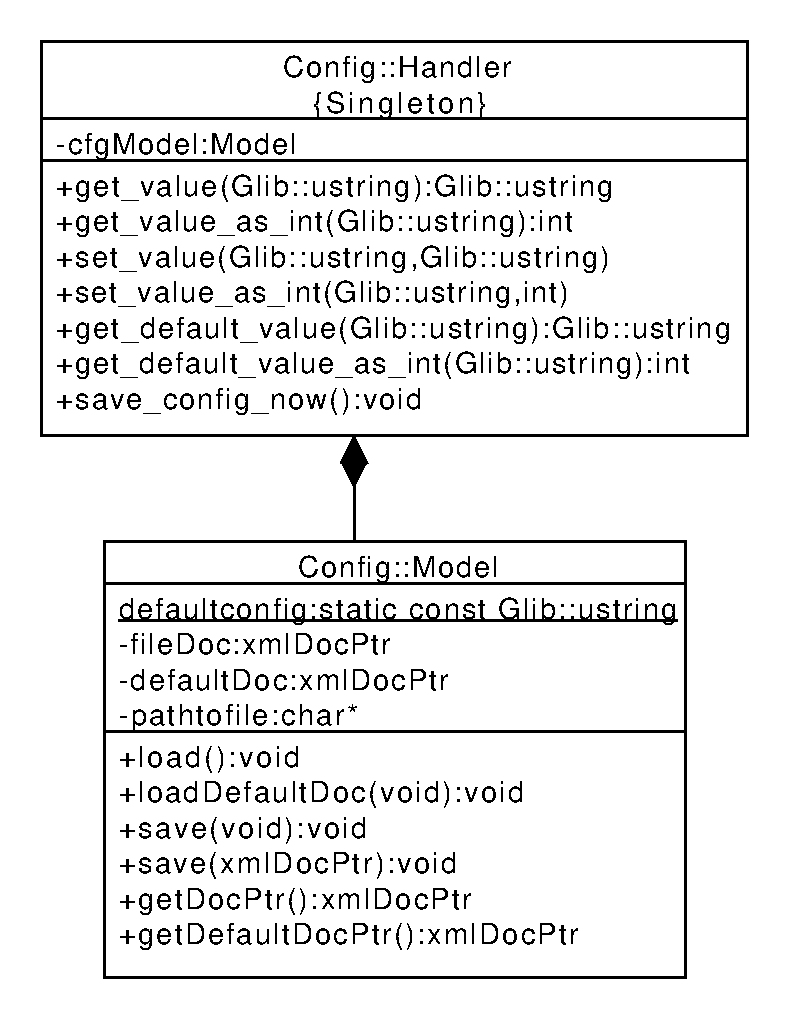
\includegraphics[scale=0.6]{./gfx/class/hand_model}
    \caption{Config-Model Beziechung}
    \label{c_confmod}
\end{figure}
Die \emph{Config::Model} Klasse gehört nach dem MVC Paradigma zur Model Schicht. Diese Klasse soll die nötigen Daten (Konfigurationsdatei)
die zum Betrieb von Freya nötig sind im Speicher vorhalten und Methoden zum Lesen und Speichern der Konfigurationsdatei auf die Festplatte bereit stellen (siehe \ref{c_confmod}).



Zum Parsen der XML Datei soll hier die C Programmbibliothek libxml2 verwendet werden. Diese Library wurde gewählt, weil sie alle benötigten Funktionen enthält, nach dem ANSI-C Standard implementiert ist
und bereits seit über einem Jahrzehnt Quasi-Standard im C Umfeld ist.

Informationen zur zu verwendenden Libaray:

    \begin{itemize}
        \item \url{http://xmlsoft.org/}
        \item \url{http://en.wikipedia.org/wiki/Libxml2}
    \end{itemize}

\begin{figure}[htb!]
    \centering
    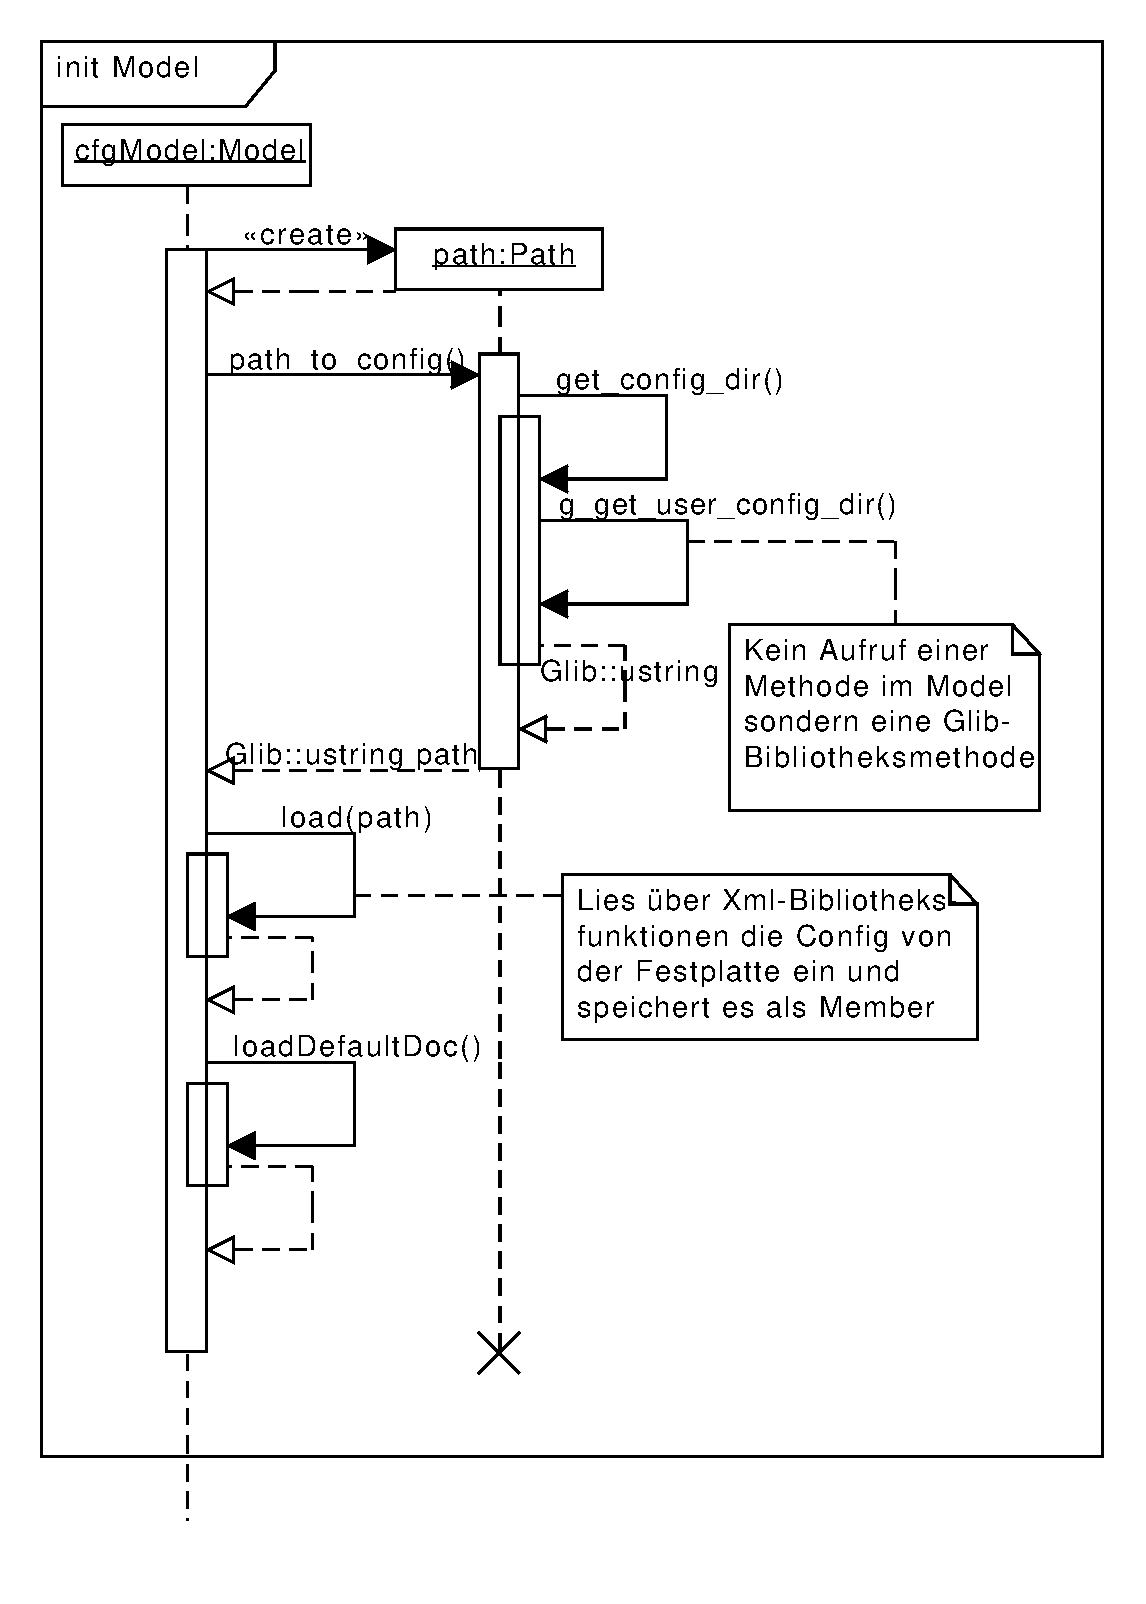
\includegraphics[scale=0.6]{./gfx/seq/init_model}
    \caption{Initialisierung des Models}
    \label{c_modelinit}
\end{figure}


\subsubsection{Instanzierung des Models}


Über die \emph{Init::Path} Klasse holt sich das Model bei seiner Instanziierung über die path\_to\_config() Methode
den Pfad zur Konfigurationsdatei, parst diese sowie die einkompilierte default Config und 
initialisiert zwei XML Document Pointer die auf ein DOM Objekt, welches einen Dokumentenbaum enthält, zeigen.
Hierzu werden die privaten load(pathtofile) und die loadDefaulDoc() Methoden der Config::Model Klasse verwendet.
\\   

Anschließend kann man über diese DOM Objekte traversieren und Werte der Konfigurationsdatei lesen oder setzten.
Die default config wurde implementiert um fehlerhaften Werten oder einer kaputten Konfiguration vorzubeugen. Ist ein benötigter Wert
nicht in der User config vorhanden oder ist diese beschädigt so wird auf die default config zurückgegriffen.
Bei Beendigung des Models wird das aktuelle Objekt als XML Konfigurationsdatei auf die Festplatte geschrieben.
Wie andere Objekte auch, nutzt das Model die Log-Klasse um zu Informationen und Fehler zu protokollieren.



\subsubsection{Prinzipieller Ablauf der load() Methode}

Beim Instanzieren ruft das Model seine load() Methode mit dem aktuellem Pfad auf.
In dieser wird als Erstes die libxml2 Methode xmlParseFile(pathtofile) aufgerufen. Diese bekommt den
Pfad zur Konfigurationsdatei übergeben und versucht über den übergebenen Pfad das File zu laden.
\\
Wenn die Operation erfolgareich war, wird ein Dokument Pointer von der xmlParseFile() 
zurückgegben, im Fehlerfall wird \emph{NULL} zurückgegeben.
\\
Anschließend wird das geladene Dokument auf Gültigkeit geprüft, zeigt dieses auf \emph{NULL} so wird eine entsprechende Fehlermeldung über den Log::Writer in die Logdatei geschreiben. Wurde ein gültiger xmlDocPtr zurückgegeben so soll folgendes passieren:

\begin{itemize}
    \item Ein Node Pointer wird auf das root Element über xmlDocGetRootElement() gesetzt
    \item Überprüfung ob Node Pointer Null ist, trifft das zu, so wird ein Error in die Logdatei geschrieben
        allokierter Speicher vom Dokument Pointer mittels xmlFreeDoc() freigegeben und dieser auf NULL gesetzet
    \item Ist der Node Pointer gültig, so wird mittels der libxml2 Methode xmlStrcmp(DocPtr, ,,freya'') geprüft ob das
        root Element ,,freya'' entspricht. Ist dies der Fall wird eine Erfolgsmeldung in die Logdatei geschreiben. Im Fehlerfall wird eine Fehlermeldung rausgeschreiben, allokierter Speicher freigegeben
        und der Dokument sowie der Node Pointer auf \emph{NULL} gesetzt. 
\end{itemize}


\subsubsection{loadDefaultDoc() Methode}
Diese Methode holt sich die default Konfigurationsdatei aus einem einkompilierten String.
Dieser String wird anschließend mittels der libxml2 xmlParseMemory() geparst und ein xmlDocPtr zurückgegeben welcher als defaultDoc Membervariable gespeichert wird.

\subsubsection{Ablauf der save() Methode}
Die save() Methode ist eine Wrapper Methode für save(char*, xmlDocPtr). Sie ruft lediglich diese mit dem aktuellen Dokument Pointer und dem Pfad zur config.xml auf.

\begin{figure}[htb!]
    Quellen zur Implementierung:
    \begin{itemize}
        \item \url{http://xmlsoft.org/tutorial/index.html}
        \item \url{http://student.santarosa.edu/~dturover/?node=libxml2}
    \end{itemize}
\end{figure}



\subsection{Handler}
Die Config::Handler Klasse gehört nach dem MVC Paradigma zur Controller Schicht. Diese Klasse soll für das Management bzw für den
Zugriff auf das Model und somit die Konfigurationsdatei zuständig sein. Sie enthält Methoden zum Lesen und Setzen der einzelnen Optionen.
\\
\\
Der Config::Handler wird als Singleton implementiert um einen zentralen Zugriff für alle anderen Programmteile über eine einzelne Schnittstelle zu ermöglichen.
\\
\\
Der Handler soll einen Pointer als Membervariable auf das aktuelle Model Objekt bekommen um direkten Zugriff auf die Dokument Pointer
zu haben. Desweiteren sollen Wrapper um die get und set value Methoden geschrieben werden um verschiedene Datentypen lesen und setzen zu können, so kann gleich eine ,,Teilvalidierung'' erfolgen.

\begin{figure}[htb!]
    Der Config::Handler stellt folgende Makros bereit:
    \begin{verbatim}
    CONFIG_SET(x,y) 
    CONFIG_GET(x)   
    CONFIG_SET_AS_INT(x,y) 
    CONFIG_GET_AS_INT(x)   
    CONFIG_SAVE_NOW() 
    CONFIG_GET_DEFAULT(x)
    CONFIG_GET_DEFAULT_AS_INT(x)
    \end{verbatim}
\end{figure}

\begin{figure}
    \centering
    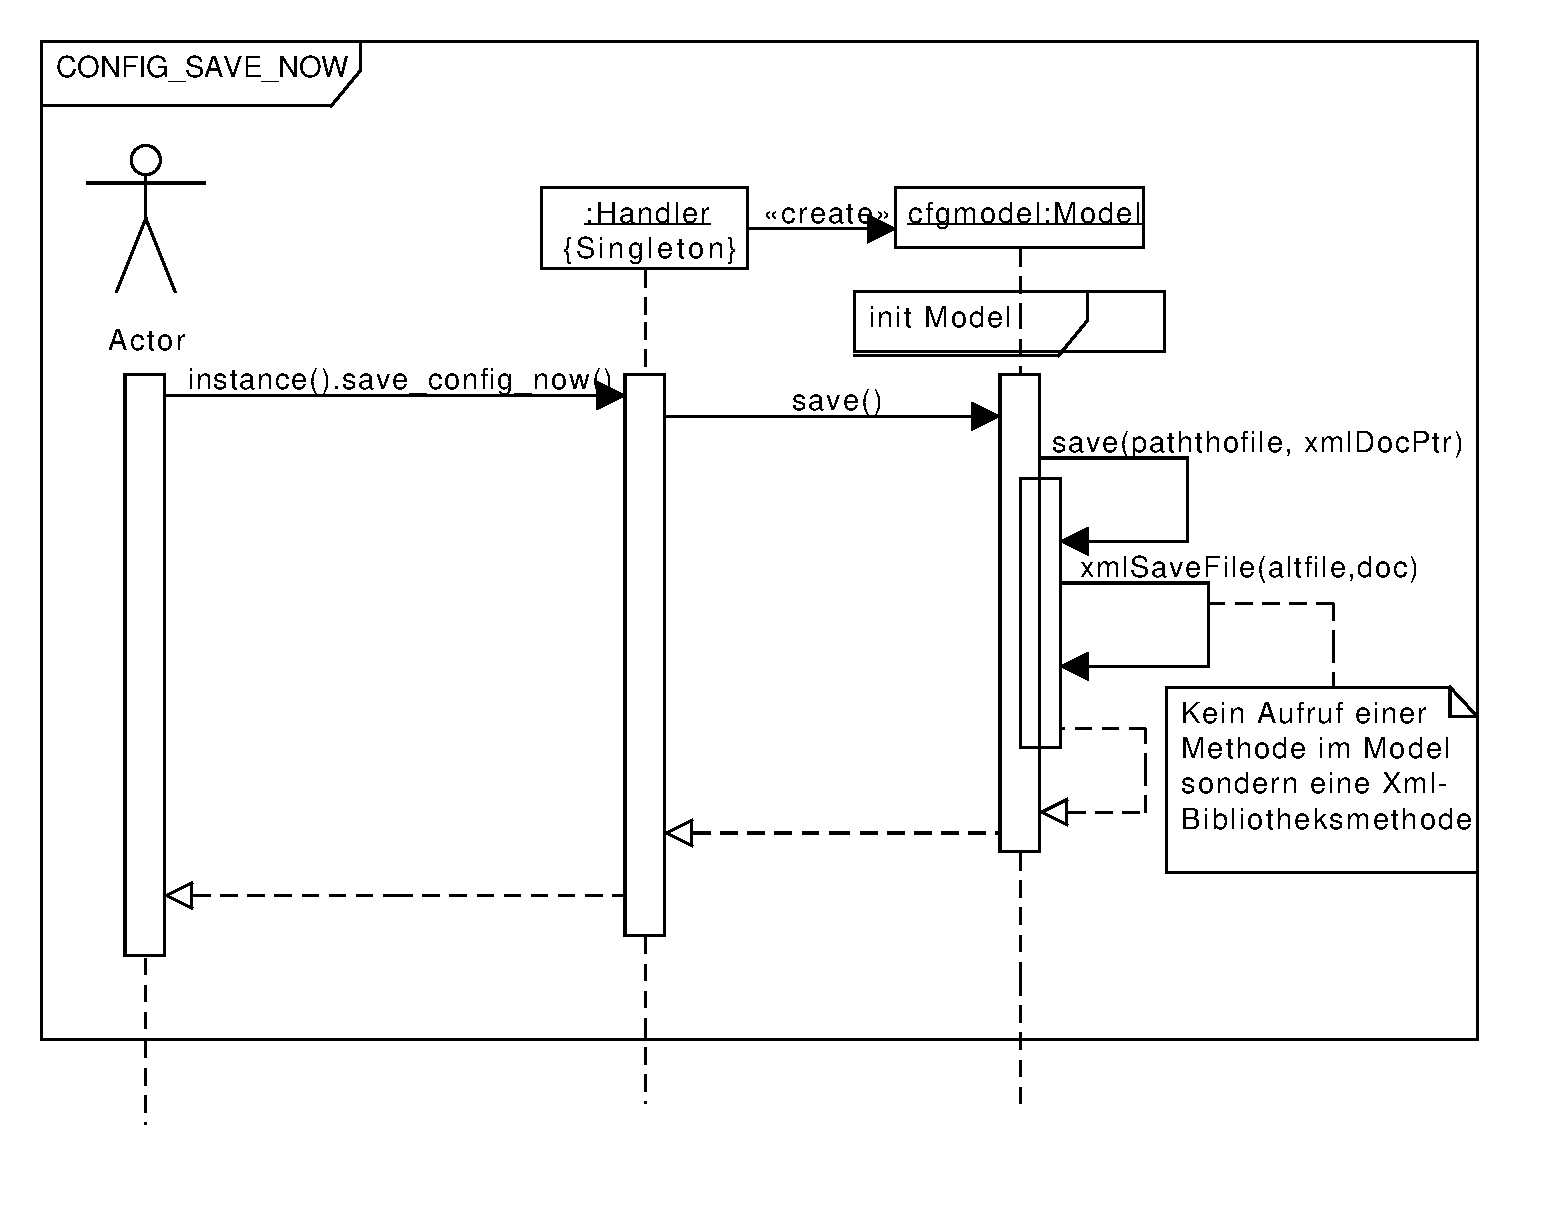
\includegraphics[scale=0.5]{./gfx/seq/config_save}
    \caption{Ablauf der Config Save Methode}
    \label{c_configsave}
\end{figure}
Über die \emph{save\_now()} Abb. \ref{c_configsave} Methode soll die aktuelle Konfiguration direkt über das Model gespeichert werden können.
Alle Methoden nutzen nach Möglichkeit Log::Writer um Informationen und Fehler in der Logdatei zu protokollieren.
\newpage
\paragraph{Grober Ablauf beim setzen einer Integer Wertes:}
\begin{figure}
    \centering
    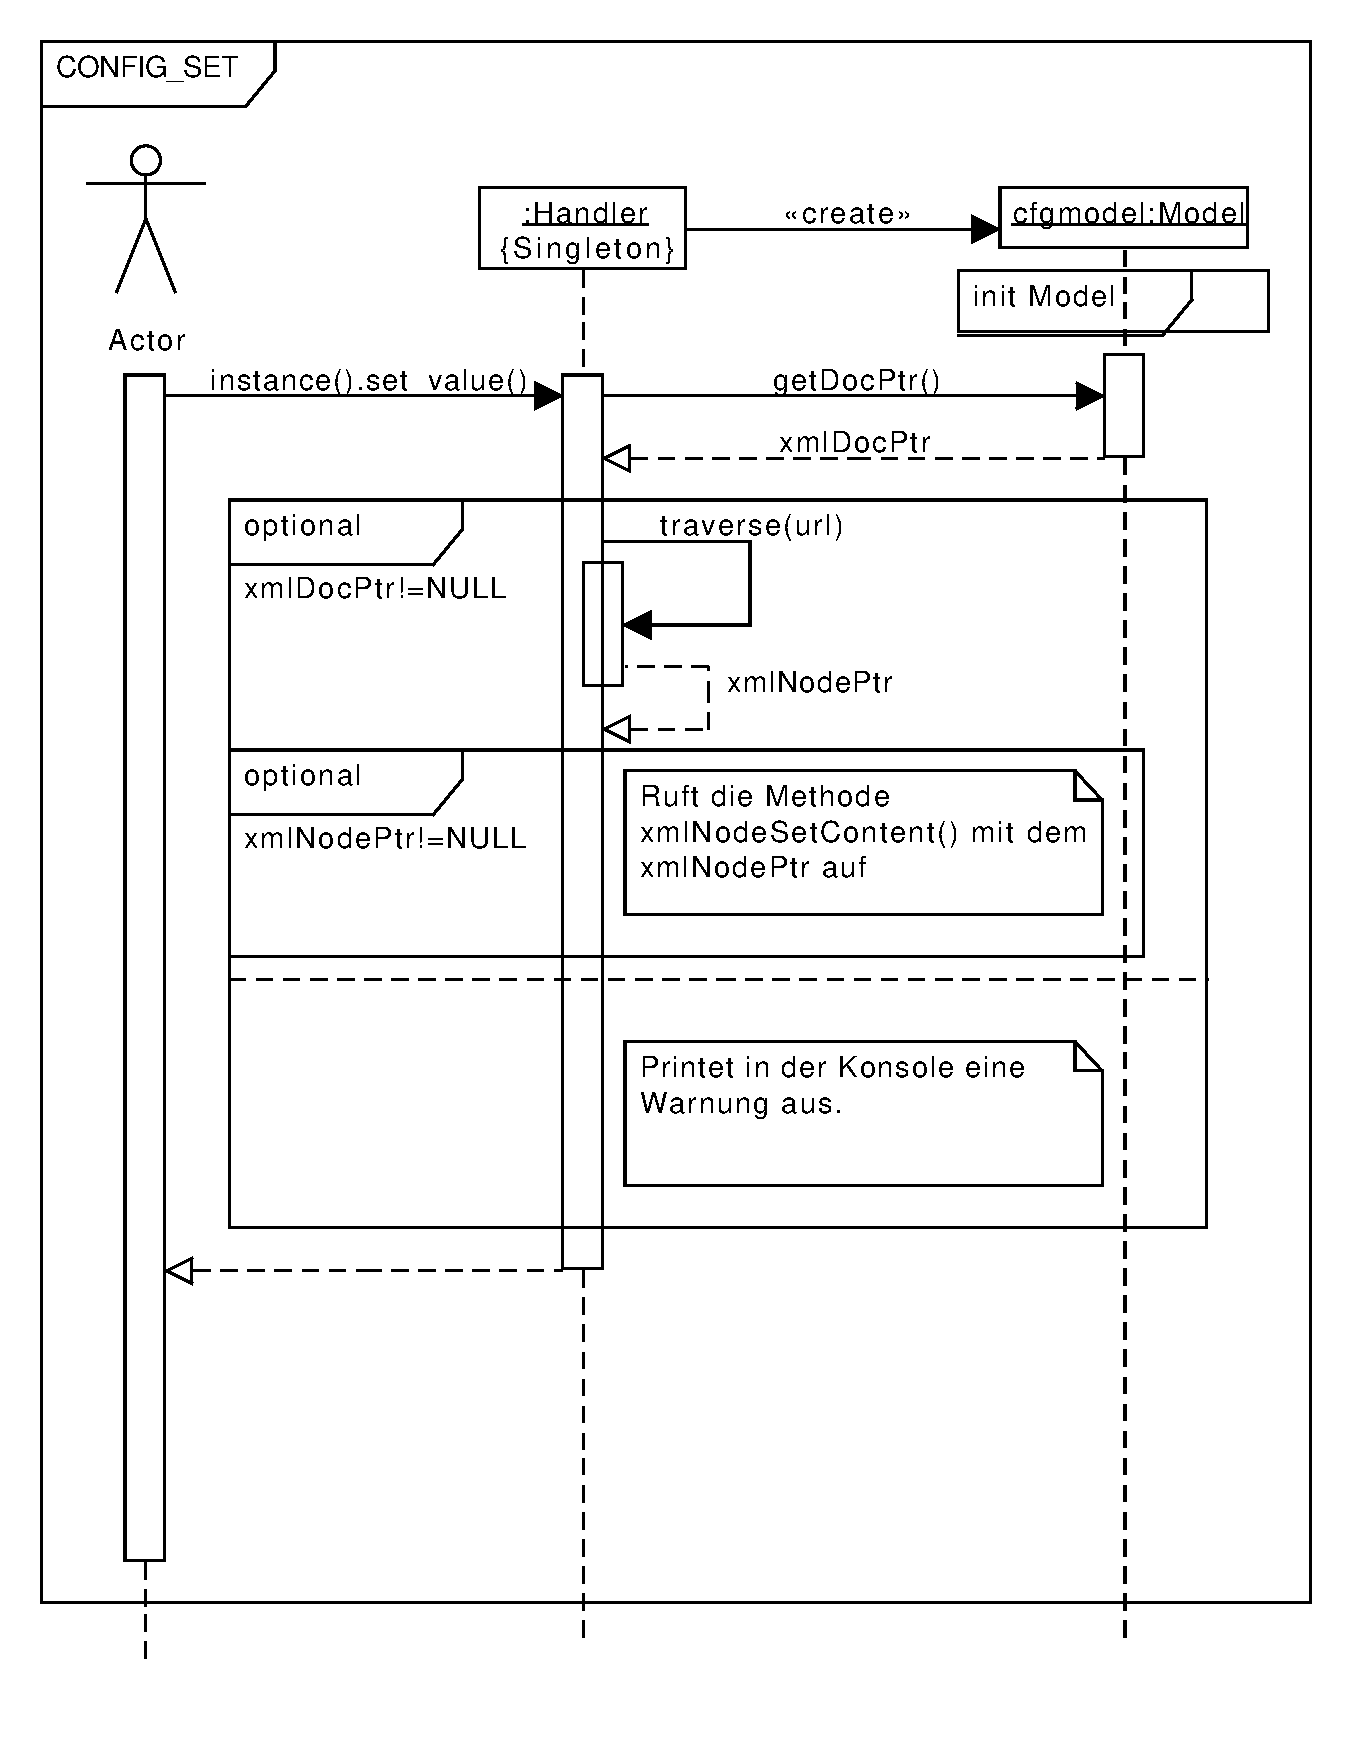
\includegraphics[scale=0.5]{./gfx/seq/config_set}
    \caption{Config set vlaue() Ablauf}
    \label{c_configget}
\end{figure}
\begin{itemize}

    \item Aufruf des \verb+CONFIG_SET_AS_INT("settings.connection.port",6667)+ Makros
    \item Über das Makro wird die Wrapper Methode \verb+set_value_as_int()+ aufgerufen
    \item Diese Methode wandelt den Integer Wert in einen String um und ruft die eigentliche set Methode set\_value(url, wert) auf
    \item Die set\_value(url, wert) Methode holt sich mit cfgmodel.getDocPtr() einen aktuellen Dokument Pointer über das Model
    \item Ist der Dokument Pointer \emph{NULL}, so kann kein Wert geschrieben werden, also wird über den Log:Writer
        eine entsprechende Warnung in die Logdatei geschreiben.
    \item Bei einem gültigem Dokument Pointer wird  mittels xmlDocGetRootElement() auf das root Element zugegriffen
    \item Anschließend wird mit xmlChildrenNode der Node Pointer auf den folgenden Kinderknoden gesetzt und die traverse() Methode aufgerufen
    \item Nun werden diverse Vorbereitungen getätigt und anschließend rekursiv im Baum nach der übergebenen
        Url gesucht. Hierbei wird jeweils der rekursive Teilstring (eins.zwei.drei) gemäß dem Url Aufbau untersucht

    \item Wird die Url nicht gefunden oder sind andere Fehler aufgetreten wird ein \emph{NULL Pointer} zurückgegeben und eine entsprechende Fehlermeldung in die Logdatei geschrieben
    \item Wird die Url gefunden, so wird ein NodePointer auf den Optionswert über die Aufruferkette an die set\_value() Methode \emph{returned}. In dieser wird dann der Wert an der entsprechende Stelle gesetzt.  
\end{itemize}
\paragraph{Grober Ablauf beim Lesen eines Wertes:}
\begin{figure}
    \centering
    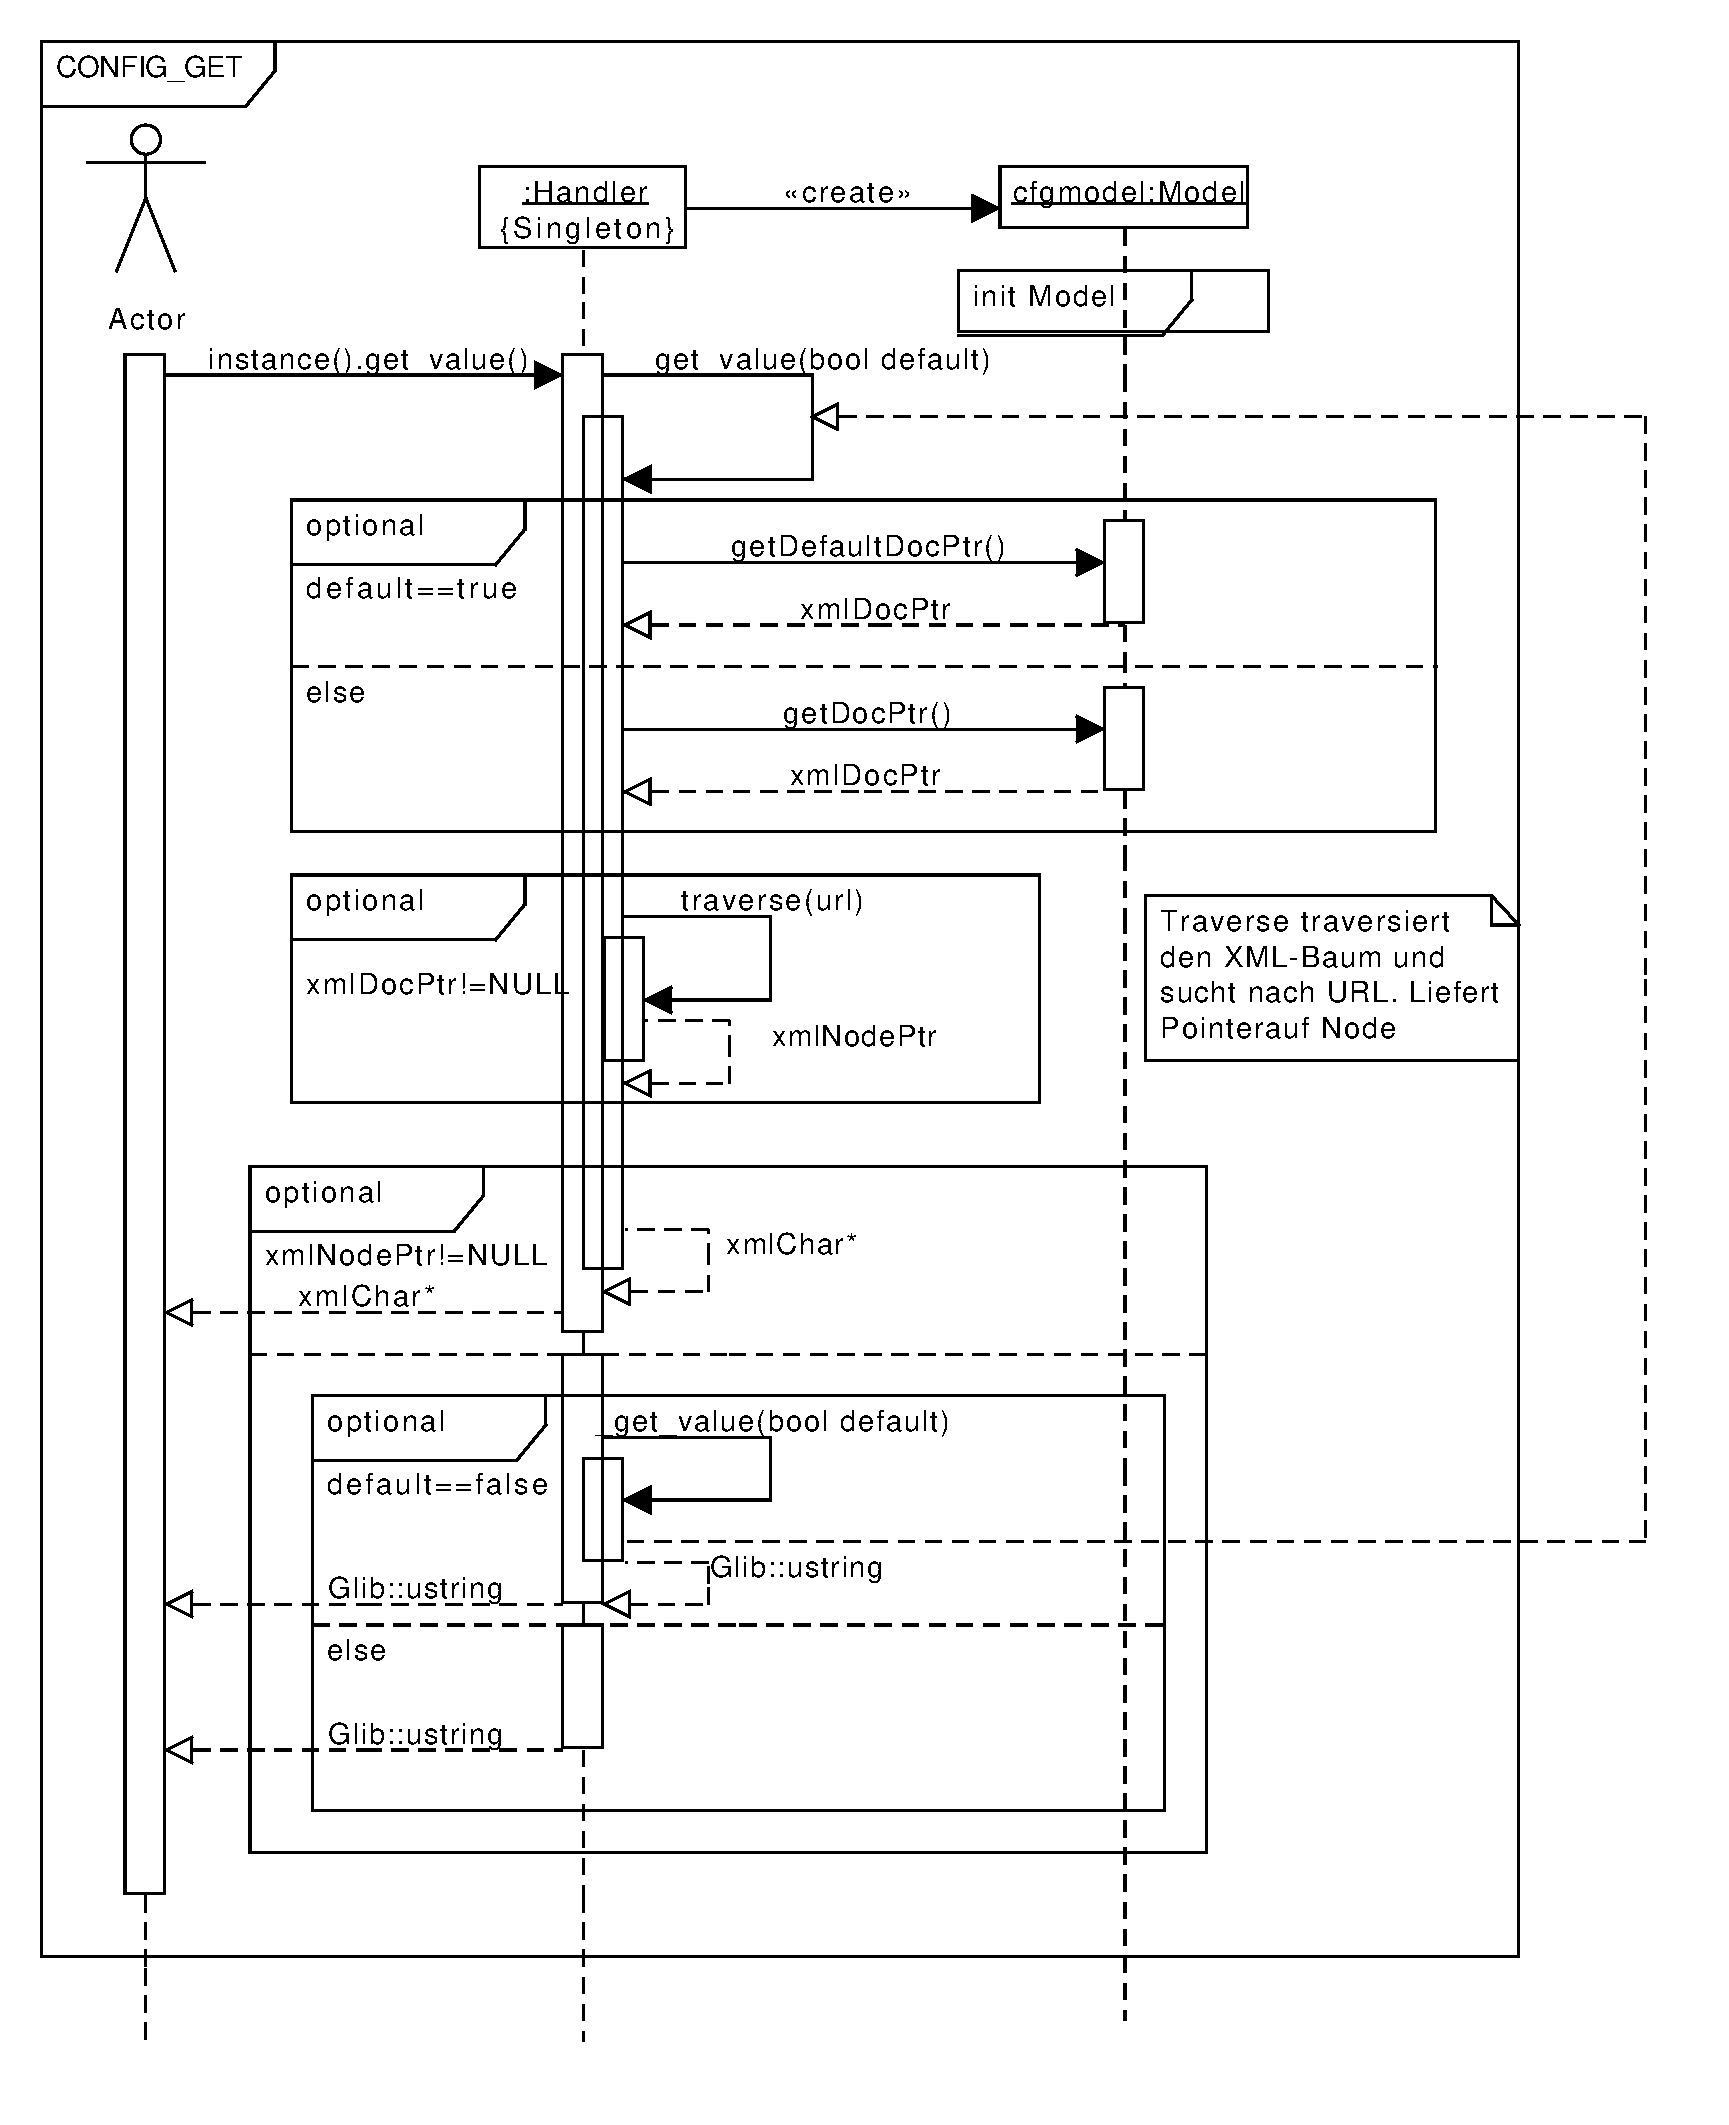
\includegraphics[scale=0.5]{./gfx/seq/config_get}
    \caption{Config get\_value() Ablauf}
    \label{c_configget}
\end{figure}
\begin{itemize}
    \item Das Makro \verb+CONFIG_GET("settings.connection.host")+ wird analog dem Setzen aufgerufen, dieses ruft die entsprechende Wrapper
        Methode get\_value() welche die eigentliche private \_get\_value() Methode aufruft.
        \\
        Der zweite Parameter dieser Methode ist ein \emph{boolean flag}, dieser dient dazu der \_get\_value()
        Methode mitzuteilen ob der entsprechende Default Wert Pointer, welcher auf die einkompilierte
        Konfigurationsdatei zeigt, oder der Custom User Config Pointer geladen werden soll.
    \item Die \_get\_value() Methode holt entsprechend dem flag, den ,,richtigen'' Dokument Pointer über das Model (analog Setzen eines Integer Wertes)
    \item Bei einen gültigen Pointer wird analog zum Setzen der Node Pointer auf das erste Element gesetzt und \textit{traverse()}
        aufgerufen (siehe Setzen eines Wertes).
    \item Kann kein Node ermittelt werden (d.h. cur Pointer zeigte auf NULL nach dem traversieren), so wird eine entsprechende Warnung in die Logdatei geschreiben.
    \item Anschließend wird die \_get\_value(url,true) Methode rekursiv mit einem \emph{true flag} aufgerufen. Aufgrund des true flags wird nun der Dokument Pointer mit den Default Werten geladen.
    \item Analog zum bisherigen Verlauf beim ,,Lesen eines Wertes'' erfolgt die Suche des Default Wertes. Kann am Ende kein
        Default Wert ermittelt werden so wird an den Aufrufer eine leerer String zurückgegeben.
\end{itemize}










